W tym rozdziale omówimy jakie jakie typy ilorazowe można zdefiniować za pomocą szeroko pojętego śladu funkcji normalizującej. Zostaną przedstawione przykłady typów indukcyjnych, których konstrukcja jest silnie inspirowana procesem ich normalizacji. Część z nich to będą już znane od dłuższego czasu typy, a inne to wymyślone na potrzeby tej pracy przykłady o różnym poziomie użyteczności.
\section{Wolne monoidy}
Osoby zajmujące się programowanie funkcyjnym czasem nazywają listy wolnymi monoidami. Nie jest to jednak oczywiste dla każdego czym są wolne monoidy a tym bardziej skąd wzięła się ta analogia.
\subsection{Czym jest wolny monoid?}
Monoid jest strukturą algebraiczną $(\mathbf{A}, \circ)$, gdzie $\mathbf{A}$ będziemy nazywać nośnikiem struktury, a $\circ$ jest działaniem w tej strukturze. O nośnikiem struktury mogą być na przykład liczby naturalne, lub jakiekolwiek inne obiekty na których możemy wykonywać działania. Działanie na strukturze jest natomiast funkcją binarną działającą na nośniku $\circ: \mathbf{A} \rightarrow \mathbf{A} \rightarrow \mathbf{A}$. Każdy monoid musi spełniać następujące prawa:
\begin{description}
\item[Element neutralny:] $\exists e \in \mathbf{A}, \forall x \in \mathbf{A}, e \circ x = x = x \circ e$
\item[Łączność działania:] $\forall x y z \in \mathbf{A}, x \circ (y \circ z) = (x \circ y) \circ z$
\end{description}
Dobrym przykładem struktury która jest monoidtem są macierze z operacją mnożenia, lub w mniej oczywisty sposób funkcje jednoargumentowe z operacją ich składania. Wolność struktury algebraicznej natomiast objawia się w tym, że ograniczymy się jedynie do do praw wynikających z jej własności, natomiast nie będziemy uwzględniać praw wynikających z jej nośnika. Zatem dla wolnego monoidu z liczbami naturalnymi jako nośnikiem nie będziemy utożsamiać z sobą wyrażeń $2$ oraz $1 + 1$, gdyż nie wynikają one z praw monoidu. Natomiast wyrażenie takie jak $(1 + 2) + 3$, będą tym samym co $1 + (2 + 3)$, gdyż łączność działania jest jednym z praw monoidu. Zatem dla dowolnego nośnika możemy myśleć o wolnym monoidzie jako drzewie operacji.
\begin{figure}[!htp]
    \centering
    \begin{tikzpicture}[sibling distance=24pt]
    \tikzset{level distance=60pt}
    \Tree [.$\circ$ [.$\circ$ a b ] [.$\circ$ c d ] ]
    \end{tikzpicture}
    \hspace{1cm}
    \begin{tikzpicture}[sibling distance=24pt]
    \Tree [.$\circ$ a [.$\circ$ b [.$\circ$ c [.$\circ$ d e ] ] ] ]
    \end{tikzpicture}

    \caption{Dwa równoważne drzewa dla wyrażenia $a \circ b \circ c \circ d$}
    \label{fig:exp_tree}
\end{figure}
\subsection{Postać normalna wolnego monalidu, czyli lista}
Jak możemy zobaczyć na rysunku \ref{fig:exp_tree} to samo wyrażenie możemy zapisać na wiele równoważnych sposobów w wolnym monoidzie, wynika to z faktu, iż nawiasy nie mają znaczenia ze względu na łączność działania, a ponad to można było dopisać dowolną ilość elementów neutralnych, które nie zmieniają wartości wyrażenia. W naiwny sposób moglibyśmy zatem zaimplementować wolny monoid korzystając z 3 konstruktorów \ref{FreeMonoid}: elementu neutralnego, dowolnej wartości, oraz łączącego ich operatora.
\begin{code}
\begin{minted}{coq}
Inductive FreeMonoid (A: Type) :=
| leaf : FreeMonoid A
| var  : A -> FreeMonoid A
| op   : FreeMonoid A -> FreeMonoid A -> FreeMonoid A.
\end{minted}
\caption{Naiwna definicja wolnego monoidu w Coqu.}
\label{FreeMonoid}
\end{code}
Taka naiwna definicja, tak jak nasze drzewa \ref{fig:exp_tree}, powoduje problem niejednoznaczności reprezentacji. Aby rozwiązać ten problem musimy ustalić jaką postać tego wyrażenia będziemy traktować jako normalną. Zastosujemy tutaj klasyczne rozwiązanie, w którym zawsze występuje dokładnie jeden element neutralny na końcu oraz operatory wiążące mocniej w lewo:
$$
    (a_1 \circ (a_2 \circ (a_3 \circ \dots  \circ (a_n \circ e) \dots ))
$$
Wprawne oko już powinno dostrzec w wyrażeniu powyżej znaną każdemu induktywną definicję listy\ref{list}, gdzie elementem neutralnym jest \mintinline{coq}{nil}, a kolejne elementy są połączone konstruktorem \mintinline{coq}{cons}.
\begin{code}
\begin{minted}{coq}
Inductive list (A: Type) :=
| nil  : list A
| cons : A -> list A -> list A.
\end{minted}
\caption{Definicja listy z biblioteki standardowej Coqa.}
\label{list}
\end{code}
Nasza funkcja normalizująca powinna zatem przechodzić po wszystkich wierzchołkach drzewa \mintinline{coq}{FreeMonoid}\ref{FreeMonoid} od lewej do prawej i przekształcać drzewo do ustalonej postaci normalnej. Ślad tej funkcji w postaci listy napotkanych elementów z pominięciem tych neutralnych jest typem ilorazowym dla wolnych monoidów. Możemy w łatwy sposób zdefiniować również funkcję która przekształci wolny monoid od razu do jego normalnej postaci w formie listy \ref{free_to_list}.
\begin{code}
\begin{minted}{coq}
Fixpoint free_to_list {A: Type} (m: FreeMonoid A) : list A :=
match m with
| leaf   => []
| var x  => [x]
| op x y => to_list x ++ to_list y
end.
\end{minted}
\caption{Definicja funkcji normalizującej wolny monoid do postaci list w Coqu.}
\label{free_to_list}
\end{code}
\section{Liczby całkowite}
Klasyczny przykładem wykorzystania typów ilorazowych są liczby całkowite. Są one naturalnym rozszerzeniem liczb naturalnych do grupy addytywnej, a więc takie w której każdy element ma swój element przeciwny. Możemy je zaimplementować w naiwny sposób za pomocą pary liczb naturalnych \ref{Int}. Liczba po prawej stronie będzie reprezentować z ilu poprzedników, a liczba po prawej stronie z ilu następników składa się definiowana liczba.
\begin{code}
\begin{minted}{coq}
Definition Int : Type := nat * nat.
\end{minted}
\caption{Naiwna reprezentacja liczb całkowitych w Coqu.}
\label{Int}
\end{code}
Taka reprezentacja jest bardzo wygodna w implementacji, takich operacji jak suma\ref{int_add}, następnik, czy poprzednik. Wynika to z faktu, że możemy w tym celu wykorzystać już istniejące operacje na liczbach naturalnych.  
\begin{code}
\begin{minted}{coq}
Definition int_add (n: Int) (m: Int) : Int :=
  let (a, b) := n in let (c, d) := m in (a + c, b + d).
\end{minted}
\caption{Dodawanie naiwnie zdefiniowanych liczb całkowitych w Coqu.}
\label{int_add}
\end{code}
Niestety taka definicja pozostawia problem niejednoznaczności reprezentacji. Żeby się na niego natknąć wystarczy porównać wyniki $1 + (-1) = 0$ oraz $2 + (-2) = 0$. Pomimo iż oba te wyrażenia mają ten sam wynik to w naiwnej postaci \mintinline{coq}{Int}\ref{Int}, będą one reprezentowane jako odpowiednio $(1, 1)$ oraz $(2, 2)$.
\subsection{Funkcja normalizująca dla liczb całkowitych}
Aby pozbyć się problemu niejednoznaczności będziemy musieli wyznaczyć postać normalną dla liczb całkowitych. W naszym przypadku za normalną uznamy postać w której przynajmniej jednym z elementów pary jest liczba zero. Funkcją normalizującą będziemy nazywać taką, która będzie odejmować jedynkę z lewej i prawej strony, tak długo, aż nie będzie to już możliwe \ref{int_norm}.
\begin{code}
\begin{minted}{coq}
Function int_norm' (x y : nat) : (nat * nat) :=
match x, y with
| S x', S y' => int_norm' x' y'
| _, _       => (x, y)
end.

Function int_norm (p: nat * nat) : (nat * nat) := 
  let (x, y) := p in int_norm' x y.
\end{minted}
\caption{Definicja funkcji normalizującej liczby całkowite w Coqu.}
\label{int_norm}
\end{code}

Po zakończeniu działania tej funkcji pozycja na której pozostanie liczba niezerowa będzie wyznaczała znak liczby całkowitej, natomiast jej wartość będzie wyznaczać wartość bezwzględną całej liczby całkowitej.
\begin{figure}[!htp]
    \centering

    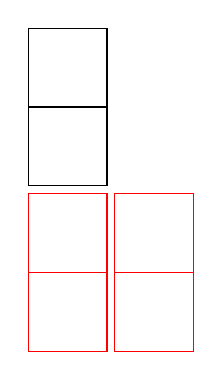
\begin{tikzpicture}
    \draw[draw=red] (0,0) rectangle ++(1,1);
    \draw[draw=red] (1.1,0) rectangle ++(1,1);
    \draw[draw=red] (0,1) rectangle ++(1,1);
    \draw[draw=red] (1.1,1) rectangle ++(1,1);
    \draw[draw=black] (0,2.1) rectangle ++(1,1);
    \draw[draw=black] (0,3.1) rectangle ++(1,1);
    \end{tikzpicture}
    \hspace{1cm}
    \begin{tikzpicture}
    \draw[draw=red] (0,0) rectangle ++(1,1);
    \draw[draw=red] (1.1,0) rectangle ++(1,1);
    \draw[draw=black] (1.1,1.1) rectangle ++(1,1);
    \draw[draw=black] (1.1,2.1) rectangle ++(1,1);
    \draw[draw=black] (1.1,3.1) rectangle ++(1,1);
    \end{tikzpicture}
    \hspace{1cm}
    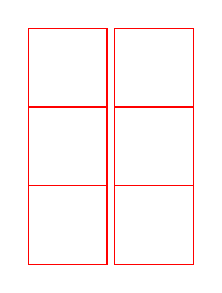
\begin{tikzpicture}
    \draw[draw=red] (0,0) rectangle ++(1,1);
    \draw[draw=red] (1.1,0) rectangle ++(1,1);
    \draw[draw=red] (0,1) rectangle ++(1,1);
    \draw[draw=red] (1.1,1) rectangle ++(1,1);
    \draw[draw=red] (0,2) rectangle ++(1,1);
    \draw[draw=red] (1.1,2) rectangle ++(1,1);
    \end{tikzpicture}

    \caption{Wizualizacja działania funkcji normalizującej dla liczb całkowitych (odpowiednio -2, 3 i 0), na czerwono zaznaczone są elementy które zostaną usunięte przez działanie tej funkcji.}
    \label{fig:int_norm}
\end{figure}
\subsection{Indukcyjny typ liczb całkowitych z jednoznaczną reprezentacją}
Mając już do dyspozycji funkcję normalizującą możemy wykorzystać idę jej działania do stworzenia typu indukcyjnego, który będzie charakteryzował się jednoznacznością reprezentacji. Sam ślad funkcji nie jest szczególnie ciekawy w tym przypadku. Możemy jednak dużo nauczyć się z ostatniego kroku procesu normalizacji. W kodzie \ref{int_norm} jest on uproszczony do \mintinline{coq}{_, _}, jednak pod tym wzorcem możemy wyróżnić trzy przypadki:
\begin{description}
    \item[\mintinline{coq}{S x', O}] - gdy wynikiem jest liczba ujemna o wartości \mintinline{coq}{S x'},
    \item[\mintinline{coq}{O, S y'}] - gdy wynikiem jest liczba dodatnia o wartości \mintinline{coq}{S y'},
    \item[\mintinline{coq}{O, O}] - gdy wynikiem jest zero.
\end{description}

Możemy zatem stworzyć typ indukcyjny z konstruktorami dla każdego z tych trzech przypadków.
\begin{code}
\begin{minted}{coq}
Inductive Z : Type :=
| Pos  : nat -> Z
| Zero : Z
| Neg  : nat -> Z.
\end{minted}
\caption{Definicja typu liczb całkowitych z jednoznaczną reprezentacją w Coqu.}
\label{Z}
\end{code}

Możemy w bardzo łatwy sposób zmodyfikować funkcję normalizującą \ref{int_norm}, na taką, która przekształca naszą naiwną reprezentację na nową, jednoznaczną. 
\begin{code}
\begin{minted}{coq}
Function int_to_Z (x y : nat) : Z :=
match x, y with
| S x', S y' => norm x' y'
| S x', O    => Neg x'
| O   , S y' => Pos y'
| O   , O    => Zero
end.
\end{minted}
\caption{Definicja funkcji przekształcającej naiwną reprezentację w jednoznaczną Coqu.}
\label{int_to_Z}
\end{code}

Taka definicja nie pozostawia wątpliwości co do swojej jednoznaczności, o ile oczywiście funkcja normalizująca jest poprawna. 
\subsection{Podstawowe operacje na jednoznacznych liczbach całkowitych}
Możemy teraz przejść do zdefiniowania kilku przykładowych funkcji dla liczb całkowitych, na zdefiniowanym powyżej typie \mintinline{coq}{Z} \ref{Z}. Tak jak w przypadku liczb naturalnych warto zacząć od rozpocząć od zdefiniowania następnika, a z racji posiadania liczb ujemnych również poprzednika.
\begin{code}
\begin{minted}{coq}
Definition succ (n: Z) : Z :=
match n with
| Pos k => Pos (S k)
| Zero => Pos O
| Neg O => Zero
| Neg (S n) => Neg n
end.
\end{minted}
\caption{Definicja następnika dla liczb całkowitych \mintinline{coq}{Z} \ref{Z}.}
\label{Z_succ}
\end{code}

\begin{code}
\begin{minted}{coq}
Definition pred (n: Z) : Z :=
match n with
| Pos (S n) => Pos n
| Pos O => Zero
| Zero => Neg O
| Neg n => Neg (S n)
end.
\end{minted}
\caption{Definicja poprzednika dla liczb całkowitych \mintinline{coq}{Z} \ref{Z}.}
\label{Z_pred}
\end{code}

\begin{code}
\begin{minted}{coq}
Definition neg (n: Z) : Z :=
match n with
| Pos k => Neg k
| Zero => Zero
| Neg k => Pos k
end.
\end{minted}
\caption{Definicja poprzednika dla liczb całkowitych \mintinline{coq}{Z} \ref{Z}.}
\label{Z_neg}
\end{code}
W obu przypadkach definicja jest dojść prosta i nie pozostawia za dużo wątpliwości co do swojej poprawności. W obu przypadkach konieczny był specjalny 4 przypadek, który odpowiada za przejście do zero. Definicja negacji jest wyjątkowo trywialna w przypadku tej reprezentacji, więc nie wymaga omówienia. Przejdziemy zatem to najważniejszej operacji na liczbach całkowitych, jaką jest dodawanie.
\begin{code}
\begin{minted}{coq}
Fixpoint map_n {A: Type} (n: nat) (f: A -> A) (x: A) : A :=
match n with
| O    => x
| S n' => f (map_n n' f x)
end.

Definition add (a b : Z) : Z :=
match a with 
| Pos n => map_n (S n) succ b
| Zero  => b
| Neg n => map_n (S n) pred b
end.
\end{minted}
\caption{Definicja dodawania dla liczb całkowitych \mintinline{coq}{Z} \ref{Z}.}
\label{Z_add}
\end{code}

W przedstawionej w tej pracy definicji dodawania \ref{Z_add} została wykorzystana funkcja pomocnicza \mintinline{coq}{map_n} \ref{Z_add}. Pozwala ona na nałożenie $n$ operacji na daną wartość. Z uwagi iż nasze liczby całkowite wykorzystują liczby naturalne oczywistym jest zdefiniowanie dodawania jako wykonanie $n$ operacji następnika, lub poprzednika jeśli liczba którą dodajemy była ujemna. Odejmowanie można w łatwy sposób zdefiować jako dodawane liczby przeciwnej. Możemy zatem zdefiniować ostania, lecz równie ważną operację mnożenia.
\begin{code}
\begin{minted}{coq}

Definition mul (a b: Z) : Z :=
match a with 
| Pos n => map_n (S n) (add b) Zero
| Zero  => Zero
| Neg n => neg (map_n (S n) (add b) Zero)
end.
\end{minted}
\caption{Definicja mnożenia dla liczb całkowitych \mintinline{coq}{Z} \ref{Z}.}
\label{Z_mul}
\end{code}

Definicja mnożenia wykorzystuje podobny mechanizm jak dodawanie, z tą różnicą, że tym razem nie dodajemy jedynki od wyniku, a całą liczbę przez którą mnożymy. Jest to dojść znana rekurencyjna definicja mnożenia, więc nie będziemy poświęcać zbyt dużo czasu na nią. Wszystkie przedstawione powyżej operacji i nie tylko, wraz z dowodami ich podstawowymi prawami, takimi jak łączność, przemienność, oraz rozdzielność mnożenia względem dodawania można znaleźć w dodatku better\_integer.v.
\section{Egzotyczne liczby całkowite}
Poprzednia definicja liczb całkowitych wydaje się być naturalnym kandydatem, z uwagi na powiązanie z funkcją normalizującą, a dodatkowo pozwala na łatwe obliczenia. Większość konkurencyjnych definicji jest bardzo podobna, czasami zamiast symetrycznych trzech konstruktorów wykorzystują one dwa i jeden z nich jest obciążony zerem. Niesmak może jednak pozostawiać fakt, iż wykorzystują one w swojej definicji liczby naturalne. Nasuwa się zatem pytanie czy można zdefiniować liczby całkowite bez odwoływania się do liczb naturalnych?
\subsection{Inne spojrzenie na normalizację}
W poprzedniej sekcji patrzyliśmy na proces normalizacji "od dołu do góry", który polegał na usuwaniu następników z obu elementów pary, aż jedna będzie zerem. Możemy jednak odwrócić ten proces tworząc pewien proces pseudo-normalizacji, skupiając się na spojrzeniu "od góry do dołu". W tym procesie będziemy zliczać ile elementów jest powyżej, nie wiedząc jednak czy zliczamy następnik, czy poprzedniki. Dopiero po osiągnięciu punktu, w którym obie wartości są takie same, będziemy w stanie zweryfikować, czy liczba jest dodatnia czy ujemna. 
\begin{figure}[!htp]
    \centering

    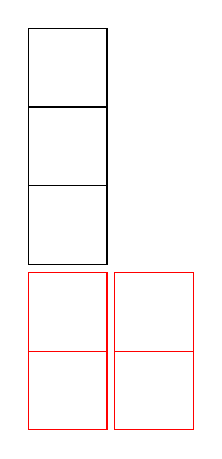
\begin{tikzpicture}
    \draw[draw=red] (0,0) rectangle ++(1,1);
    \draw[draw=red] (1.1,0) rectangle ++(1,1);
    \draw[draw=red] (0,1) rectangle ++(1,1);
    \draw[draw=red] (1.1,1) rectangle ++(1,1);
    \draw[draw=black] (0,2.1) rectangle ++(1,1);
    \draw[draw=black] (0,3.1) rectangle ++(1,1);
    \draw[draw=black] (0,4.1) rectangle ++(1,1);
    \end{tikzpicture}
    \hspace{1cm}
    \begin{tikzpicture}[grow'=down]
    \tikzset{level distance=30pt}
    \Tree [.Next [.Next [.Next Negative ] ] ]
    \draw[draw=white] (0,-4.6) rectangle ++(1,1);
    \end{tikzpicture}

    \caption{Wizualizacja działania pseudo-normalizacji "od góry do dołu".}
    \label{fig:int_psudonorm}
\end{figure}
\subsection{Następniko-poprzednik jako ślad pseudo-normalizacji}
Możemy teraz stworzyć typ iniektywny bazujący na śladzie zaprezentowanej pseudo-normalizacji. Żeby jednak był on jednoznaczny poprzebujemy pozbyć się problemu zera. W zaprezentowanej powyżej intuicji nie wiadomo w jaki sposób powinno być one reprezentowane, gdyż sytuacja w której zaczynamy od równych wartości żadna wartość nie jest większa, a więc nie wiadomo którego konstruktora użyć. Ten problem rozwiążemy zaburzając symetrię między konstruktorami. Jeden z nich będzie reprezentować zero, i w jego kontekście \mintinline{coq}{Next} będzie następnikiem, a więc \mintinline{coq}{Next Zero} będzie reprezentować jedynkę. Drugi natomiast będzie minus jedynką, a \mintinline{coq}{Next} zaaplikowany na nim będzie oznaczać poprzednik.

\begin{code}
\begin{minted}{coq}
Inductive Z' : Type :=
| Zero     : Z'
| MinusOne : Z'
| Next     : Z' -> Z'.
\end{minted}
\caption{Definicja liczby całkowitych z następniko-poprzednikiem.}
\label{Z'}
\end{code}
\subsection{Operacje na liczbach z następniko-poprzednikiem}
Konstrukcja liczb z następniko-poprzednikiem pozwala na jednoznaczną reprezentację, nie jest jednak zbyt wygodna do przeprowadzania obliczeń. Podstawowe operacje takie jak następnik, czy poprzednik mają liniową złożoność obliczeniową względem wielkości liczby. Wszystko za sprawą faktu, że aby wiedzieć czy powinniśmy dodać następniko-poprzednik czy go usunąć musimy wiedzieć czym on tak naprawdę jest, a więc musimy sprawdzić ostatni konstruktor.
\begin{code}
\begin{minted}{coq}
Function succ (k : Z') : Z' :=
match k with
| Zero => Next Zero
| MinusOne => Zero
| Next Zero => Next (Next Zero)
| Next MinusOne => MinusOne
| Next k' => Next (succ k')
end.
\end{minted}
\caption{Definicja następnika liczb całkowitych z następniko-poprzednikiem \ref{Z'}.}
\label{Z'_succ}
\end{code}
\begin{code}
\begin{minted}{coq}
Function pred (k : Z') : Z' :=
match k with
| Zero => MinusOne
| MinusOne => Next MinusOne
| Next Zero => Zero
| Next MinusOne => Next (Next MinusOne)
| Next k' => Next (pred k')
end.
\end{minted}
\caption{Definicja poprzednika liczb całkowitych z następniko-poprzednikiem \ref{Z'}.}
\label{Z'_pred}
\end{code}

Oczywiście bardziej zaawansowane operacje jak dodawanie czy mnożenie można zdefiniować, lecz definicje te nie są szczególnie przyjemne. Pominiemy je zatem w tej pracy. Definicję dodawania wraz z dowodem na izomorfizm pomiędzy tą definicją liczb całkowitych, a tą nieco bardziej klasyczną zaprezentowaną w poprzedniej sekcji możemy znaleźć w dodatku integer\_izo.v.
\section{Dodatnie liczby wymierne}
W przeciwieństwie do liczb całkowitych znalezienie jednoznacznej reprezentacji dla liczb wymiernych nie jest prostym zadanie. Ta sekcja jest operta na pracy Yves Bertot'a \cite{Qplus} w której przedstawił koncept reprezentowania liczb wymiernych za pomocą śladu algorytmu Euklidesa.
\subsection{Normalizacja liczb wymiernych}
Korzystając z podstawowej wiedzy na temat ułamków wiemy, że istnieje nieskończenie wiele reprezentacji tego samego ułamka. Zapisy takie jak $\frac{1}{2}$, $\frac{2}{4}$, czy $\frac{50}{25}$ wyrażają taką samą wartość: pół. Za postać normalną z reguły uznaje taką formę, w której nie można dokonać już operacji skrócenia ułamka, czyli podzielenia jego licznika i mianownika przez tą samą liczbę. Aby poznać przez jaką liczbę należy podzielić obie strony ułamka, aby uzyskać postać nieskracalną należy wyliczyć największy wspólny dzielnik. Jednym ze sposobów na jego wyznaczenie, jest właśnie postępowanie zgodnie z algorytmem Euklidesa \ref{euclid}. 
\begin{code}
\begin{minted}{coq}
Function euclid (p q: nat) : nat :=
match compare p q with
| Eq => p
| Gt => euclid (p - q) q n'
| Lt => euclid p (q - p) n'
end.
\end{minted}
\caption{Definicja klasycznego algorytmu Euklidesa w pseudo Coqu.}
\label{euclid}
\end{code}
Algorytm ten bazuje na prawie $\textrm{NWD}(a, b) = \textrm{NWD}(a - b, b)$, jeśli $a > b$. Inną ciekawą obserwacją z której skorzystamy, jest to że ślad algorytmu nie zmieni się, jeśli przemnożymy obie liczby przez dowolną dodatnią liczbę naturalną, w przykładzie poniżej $k$.

\begin{equation}
    \begin{split}
        11k&>5k\\
        (11-5)k=6k&>5k\\
        (6-5)k=k&<4k\\
        k&<3k=(4-1)k\\
        k&<2k=(3-1)k\\
        k&=k=(2-1)k
    \end{split}
\end{equation}

Jak widzimy w przykładzie powyżej ślad, czyli to która liczba okazała się większa nie zależy od wybranego $k$. Jedyne co się zmieniło to wyliczony największy wspólny dzielnik został przemnożony przez stałą $k$. Dodatkowo znając ślad możemy odtworzyć argumenty, z dokładnością do największego wspólnego dzielnika. Możemy zatem użyć tych śladów do jednoznacznego reprezentowania liczb wymiernych. Dowód tego faktu, jak i innych związanych z śladami algorytmów Euklidesa możemy znaleźć w dodatku Qplus.v. 
\subsection{Typ liczb wymiernych dodatnich}
Zdefiniujmy zatem typ śladów algorytmu Euklidesa \ref{Qplus}.
\begin{code}
\begin{minted}{coq}
Inductive Qplus : Type :=
| One : Qplus
| N   : Qplus -> Qplus
| D   : Qplus -> Qplus.
\end{minted}
\caption{Definicja typu śladów algorytmu Euklidesa w Coqu.}
\label{Qplus}
\end{code}
Jak mogliśmy się spodziewać składa się on z trzech konstruktorów: \mintinline{coq}{N} kiedy licznik jest większy od mianowania, \mintinline{coq}{D} gdy mianownik jest większy, oraz \mintinline{coq}{One} gdy obie wartości były równe, co zakończyło proces normalizacji. Taka konstrukcja dodatkowo zapewnia nam przyjazną indukcję po wszystkich dodatnich liczbach wymiernych, w przeciwieństwie do naiwnej reprezentacji \ref{Q} wykorzystującej parę liczb naturalnych.
\begin{code}
\begin{minted}{coq}
Definition Q : Type := (nat * nat).
\end{minted}
\caption{Definicja naiwnej reprezentacji liczb wymiernych w Coqu.}
\label{Q}
\end{code}
\subsection{Funkcje przejścia między reprezentacjami}
Wiedząc że \mintinline{coq}{Qplus} \ref{Qplus} reprezentuje ślady algorytmu Euklidesa powinniśmy być w stanie w miarę łatwo napisać kod funkcji go generującej. Niestety rzeczywistość Coqa jest dojść brutalna i termination checker nie potrafi wyznaczyć dobrze ufundowanego porządku na argumentach algorytmu Euklidesa. My wiemy że jest nim suma argumentów, lecz przekracza to jego automatyczne możliwości. Posłużymy się zatem konceptem zwanym paliwem. Polega on na dodaniu dodatkowego parametru funkcji, który będzie się zmniejszał z każdym wywołaniem rekurencyjnym funkcji, gwarantując terminację w oczach Coqa. Ustalając wartość tego parametru dostatecznie wysoko, będziemy mogli wyliczyć ślad zanim skończy nam się paliwo.
\begin{code}
\begin{minted}{coq}
Function qplus_c' (p q n: nat) : Qplus :=
match n with
| O    => One
| S n' => match compare p q with
          | Eq => One
          | Gt => N (qplus_c' (p - q) q n')
          | Lt => D (qplus_c' p (q - p) n')
          end
end.

Function qplus_c (x: Q) : Qplus :=
  let (p, q) := x in qplus_c' p q ((p + q) / gcd p q).
\end{minted}
\caption{Definicja funkcji przekształcającą naiwną reprezentację w ilorazowy typ dodanych liczb wymiernych w Coqu.}
\label{qplus_c}
\end{code}

Jak widzimy w definicji funkcji \ref{qplus_c} paliwo zostało ustalone jako suma argumentów podzielona przez ich największy wspólny dzielnik. Wiemy, że w każdej iteracji algorytm Euklidesa zmniejsza sumę argumentów przynajmniej o ich największy wspólny dzielnik, mamy zatem pewność że zdążymy wyliczyć cały ślad tego algorytmu.

Funkcja odwrotna (z dokładnością do NWD) do zaprezentowanej powyżej ma równie oczywistą konstrukcję. Będziemy odwracać proces poprzez dodawanie wartości drugiego argumentu do tego który w trakcie normalizacji był większy. Wynika to z dojść oczywistego faktu, że $(p - q) + q = p$.
\begin{code}
\begin{minted}{coq}
Function qplus_i (x : Qplus) : Q :=
match x with
| One  => (1, 1)
| N x' => let (p, q) := qplus_i x' in (p + q, q)
| D x' => let (p, q) := qplus_i x' in (p, p + q)
end.
\end{minted}
\caption{Definicja funkcji przekształcającą ilorazowy typ dodanych liczb wymiernych do naiwnej reprezentacji w Coqu.}
\label{qplus_c}
\end{code}
\subsection{Rozszerzenie do ciała liczb wymiernych}
Same dodatnie liczby wymierne nie są aż tak użyteczne jak całe ciało liczb wymiernych. Na szczęście istnieje prosty sposób na rozszerzenie tego konceptu, do wszystkich liczb wymiernych. Skorzystamy tutaj z konstrukcji podobnej do tej zaprezentowanej przy liczbach, a więc dodamy typ z trzema konstruktorami: dla liczb dodatnich, dla ujemnych oraz dla zera.
\begin{code}
\begin{minted}{coq}
Inductive FullQ :=
| Pos  : Qplus -> FullQ
| Zero : FullQ
| Neg  : Qplus -> FullQ.
\end{minted}
\caption{Definicja ilorazowego typu liczb wymiernych w Coqu.}
\label{FullQ}
\end{code}
\subsection{Operacje na liczbach wymiernych}
TODO


\section{Wolne grupy}
W tym rozdziale poznaliśmy już wolne monoidy, teraz przyszedł czas na ich bardziej skomplikowaną wersję, czyli grupy. Ma ona trzy podstawowe prawa: istnienie elementu neutralnego, łączność działania oraz istnienie elementu przeciwnego.
\begin{description}
\item[Element neutralny:] $\exists e \in \mathbf{A}, \forall x \in \mathbf{A}, e \circ x = x = x \circ e$
\item[Łączność działania:] $\forall x y z \in \mathbf{A}, x \circ (y \circ z) = (x \circ y) \circ z$
\item[Element odwrotny:] $\forall x \in \mathbf{A}, \exists x^{-1} \in \mathbf{A}, x \circ x^{-1} = x^{-1} \circ x = e$
\end{description}
Jak więc możemy zaobserwować każda grupa jest również monoidem, a jedyne co się zmienia to nowa operacja odwrotności. Jak więc możemy się domyślać wolną grupą będą listy z elementami oraz ich odwrotnościami. Naiwną implementację możemy zatem zapisać jako listę par elementu z boolem, który będzie przechowywać informację czy to ten element czy element do niego odwrotny.  
\begin{code}
\begin{minted}{coq}
Definition CanonFreeGroup (A: Type) := list (bool*A).
\end{minted}
\caption{Naiwna implementacja wolnej grupy w Coqu.}
\label{CanonFreeGroup}
\end{code}
\subsection{Normalizacja wolnej grupy}
Od normalizowanej wolnej grupy będziemy wymagać, aby dwa wzajemnie odwrotne elementy nie były swoimi sąsiadami, gdyż jak wiemy z praw grupy takie elementy się "anihilują" i są równoważne elementowi neutralnemu. 
\begin{code}
\begin{minted}{coq}
Inductive Normalized {A: Type} `{Group A} : CanonFreeGroup A -> Prop :=
| NNil   : Normalized []
| NSingl : forall (b : bool) (v : A), Normalized [(b, v)]
| NCons  : forall (b b': bool) (v v' : A) (x: CanonFreeGroup A), 
            v <> v' \/ b = b' -> Normalized ((b', v') :: x) ->
            Normalized ((b, v) :: (b', v') :: x).
\end{minted}
\caption{Predykat bycia w postaci normalnej dla wolnej grupy w Coqu.}
\label{Normalized}
\end{code}
Predykat bycia w postaci normalnej możemy wyrazić za pomocą typu induktywnego z trzema konstruktorami dla pustej grupy, singletona, oraz dla następnika \ref{Normalized}. Funkcję normalizującą\ref{normalize} również bez większych problemów da się wyrazić, jednak, żeby to zrobić nasz typ bazowy będzie musiał posiadać zdefiniowaną rozstrzygalną równość na naszym typie bazowym, w postaci funkcji \mintinline{coq}{eqf}.
\begin{code}
\begin{minted}{coq}
Class Group (A : Type) := GroupDef {
  zero      : A;
  op        : A -> A -> A;
  inv       : A -> A;
  eqf       : A -> A -> bool;
  left_id   : forall x: A, op zero x = x;
  right_id  : forall x: A, op x zero = x;
  left_inv  : forall x: A, op (inv x) x = zero;
  right_inv : forall x: A, op x (inv x) = zero;
  op_assoc  : forall x y z: A, op (op x y) z = op x (op y z);
  eqf_eq    : forall x y, reflect (x = y) (eqf x y)
}.
\end{minted}
\caption{Klasa grup z rozstrzygalną równością w Coqu.}
\label{normalize}
\end{code}

\begin{code}
\begin{minted}{coq}
Fixpoint normalize {A: Type} `{Group A} (x: CanonFreeGroup A) :=
match x with
| [] => []
| (b, v) :: x' => 
    match normalize x' with
    | [] => [(b, v)]
    | (b', v') :: x'' => if andb (eqf v v') (xorb b b')
                         then x''
                         else (b, v) :: (b', v') :: x''
    end
end.
\end{minted}
\caption{Funkcja normalizująca wolną grupą w Coqu.}
\label{normalize}
\end{code}
\subsection{Jednoznaczny typ dla wolnych grup w Coqu}
Wiedząc już czym charakteryzują się wolne grupy znormalizowane, możemy przejść do stworzenia typu induktywnego dla nich bazując na funkcji normalizacji. Pierwszą ważną obserwacją jest to, że funkcja zaczyna swoją normalizację od końca, wyznaczając element początkowy. Pod drugie wyrażenie \mintinline{coq}{eqf v v'} jest równoważne przyrównaniu do elementu neutralnego, różnicy  \mintinline{coq}{v} oraz \mintinline{coq}{v'}, czyli \mintinline{coq}{eqf (op v (inv v')) zero}. A więc tak naprawdę interesują nasz różnice między elementami. Po trzecie podobnie jak w przypadku elementów, tu również interesują nasz różnice między kolejnymi znakami. Nasz typ ilorazowy będzie zatem odwrotną listą różnicową elementów i ich znaków, czyli taką w której różnice odnoszą się do poprzedniego elementu, z dodatkowym warunkiem zabezpieczającym przed postawieniem dwóch tych samych elementów z innym znakiem obok siebie.
\begin{code}
\begin{minted}{coq}
Inductive NonEmptyFreeGroup (A: Type) `{Group A} :=
| Singl  : bool -> A -> NonEmptyFreeGroup A
| Switch : forall x: A, Squash (x <> zero) -> NonEmptyFreeGroup A -> NonEmptyFreeGroup A
| Stay   : A -> NonEmptyFreeGroup A -> NonEmptyFreeGroup A.

Definition FreeGroup (A: Type) `{Group A} := option (NonEmptyFreeGroup A).
\end{minted}
\caption{Ilorazowy typ wolnej grupy w Coqu.}
\label{FreeGroup}
\end{code}

Jak widzimy w definicji \ref{FreeGroup} mamy tak naprawdę dwa typy, pustych oraz nie pustych list wolnych. Wynika to z problemu niejednoznaczności dla elementu neutralnego (pustej grupy). Odwrotnością elementu neutralnego jest on sam, a więc zgodnie z prawami nie powinna istnieć pusta grupa "dodatnia" oraz "ujemna", stąd też potrzeba zdefiniowania niepustej wolnej grupy. Sama jej definicja składa się z trzech konstruktorów. Singleton jest dojść prostym konstruktorem bez niespodzianek. Drugi konstruktor natomiast reprezentuje zmianę znaku w stosunku do poprzedniego elementu, w związku z tym wymaga on aby różnica elementów była różna od 0, gdyż w przeciwnym wypadku obok siebie stałyby te same elementy z przeciwnymi znakami. Żeby nie martwić się o jednoznaczność dowodu został on opakowany w \mintinline{coq}{Squash} a więc żyje w świecie z definicyjną irrelewancją dowodów. Ostatni z konstruktorów reprezentuje różnicę bez zmiany znaków, w takim wypadku nie są potrzebne dodatkowe dowody, a więc jest on dojść prosty. Niestety, wymaganie odnośnie wyliczania różnicy wymusza, aby typ bazowy był sam w sobie grupą z operacją odwrotności.
\subsection{Funkcje przejścia między reprezentacjami}
Mając już zdefiniowany typ ilorazowy dla wolnych list powinniśmy zdefiniować funkcję która pozwoli nam przekonwertować naszą nawianą reprezentację do typu ilorazowego. Jej definicja nie jest zupełnie trywialne ze względu na zastosowany typ zależny w drugim konstruktorze.
\begin{code}
\begin{minted}{coq}
Fixpoint to_uniq' {A: Type} `{Group A} (b : bool) (v: A) (x: CanonFreeGroup A) 
: NonEmptyFreeGroup A :=
match x with 
| []             => Singl b v
| (b', v') :: x' => 
    if eqb b b' 
    then Stay (sub v v') (to_uniq' b' v' x')
    else match eqf_eq (sub v v') zero with
         | ReflectF _ p => Switch (sub v v') (squash p) (to_uniq' b' v' x')
         | _  => (Singl b v) (* invalid *)
         end
end.

Definition to_uniq {A: Type} `{Group A} (x: CanonFreeGroup A) : FreeGroup A :=
match x with
| [] => None
| (b, v) :: x' => Some (to_uniq' b v x')
end.
\end{minted}
\caption{Definicja funkcji przekształcającej naiwną reprezentacje w ilorazową w Coqu.}
\label{to_uniq}
\end{code}

Jak widzimy w definicji funkcji \mintinline{coq}{to_uniq} \ref{to_uniq}, w przypadku w którym zmieniamy znak musimy wyciągnąć dowód, że dwa kolejne elementy są od siebie różne. Na szczęście użycie \mintinline{coq}{reflect} w definicji grupy pozwala nam w łatwy sposób wyciągnąć taki dowód, jeśli funkcja \mintinline{coq}{eqf} zwraca \mintinline{coq}{false}. W przeciwnym zaś przypadku funkcja zwraca cokolwiek. Wprawne oko pozwala wypatrzeć, że funkcja \mintinline{coq}{to_uniq} działa poprawnie tylko dla znormalizowanych wolnych grup, jeśli chcemy pozbyć się tego ograniczenia należy ją złożyć z funkcją normalizującą \mintinline{coq}{normalize} \ref{normalize}.

\begin{code}
\begin{minted}{coq}
Fixpoint to_canon' {A: Type} `{Group A} (x: NonEmptyFreeGroup A) : CanonFreeGroup A :=
match x with 
| Singl b v     => [(b, v)]
| Stay v x'     => match to_canon' x' with
                   | [] => [(true, v)] (* invalid *)
                   | (b, v') :: y => (b, op v v') :: (b, v') :: y
                   end
| Switch v _ x' => match to_canon' x' with
                   | [] => [(true, v)] (* invalid *)
                   | (b, v') :: y => (negb b, op v v') :: (b, v') :: y
                   end
end.

Definition to_canon {A: Type} `{Group A} (x: FreeGroup A) : CanonFreeGroup A :=
match x with
| None => []
| Some x' => to_canon' x'
end.
\end{minted}
\caption{Definicja funkcji przekształcającej ilorazową reprezentacje w naiwną w Coqu.}
\label{to_canon}
\end{code}

Funkcja odwrotna \mintinline{coq}{to_canon} \ref{to_canon} ma nieco prostszy kod, gdyż nie wymaga ona tworzenia typów zależnych. Cała jej idea skupia się dodawania zapisanej różnicy do poprzedniego elementu i dzięki temu wyliczanie kolejnych wartości wolnej grupy.
\subsection{Wolna grupa jako grupa}

\subsection{Wolna grupa jako monada}
\subsection{Zastosowania wolnych grup}
\section{Listy różnicowe jak multi-zbiory}
W poprzednim rozdziale pokazaliśmy jak można zdefiniować zbiry i multi-zbiory w Coqu używając pod-typowania. Jest to skuteczna strategia, której niestety nie da się przenieść do języków nie posiadających typów zależnych takich jak Haskell. Nasuwa się zatem pytanie czy istnieją typy bazowe dla których można zdefiniować multi-zbiory bez wykorzystania pod-typowania. W tym celu wykorzystamy listę różnic pomiędzy kolejnymi elementami multi-zbioru.
\subsection{Funkcja normalizująca}
Jak można się domyślać w celu normalizacji listy elementów w multi-zbiór posłużymy się funkcją sortującą, podobnie jak w poprzednim rozdziale. 
\begin{code}
\begin{minted}{coq}
Fixpoint min (h: nat) (l: list nat) : nat :=
match l with
| [] => h
| (h' :: l') => if h' <=? h then min h' l' else min h l'
end.

Fixpoint sub_list (s: nat) (l: list nat) : list nat :=
match l with
| [] => []
| (h :: l') => (h - s) :: sub_list s l'
end.

Fixpoint rm_one_zero (l: list nat) : list nat :=
match l with
| [] => []
| (h :: l') => if h =? O then l' else h :: rm_one_zero l'
end.

Fixpoint select_sort' (f: nat) (prev: nat) (l : list nat) : list nat :=
match f with
| O => []
| S f' =>
  match l with
  | [] => []
  | (h :: l') => let m := min h l' in
                 let p := prev + m in
                 p :: (select_sort' f' p (rm_one_zero (sub_list m l)))
  end
end.

Definition select_sort (l : list nat) : list nat :=
  select_sort' (length l) O l.
\end{minted}
\caption{Definicja sortowania przez wybieranie dla liczb naturalnych w Coqu.}
\label{select_sort}
\end{code}
Tutaj w jednak przyjrzymy się pewnemu zmodyfikowanemu algorytmowi sortowanie przez wybieranie dla liczb naturalnych \ref{select_sort}. Modyfikacja ta polega na zoptymalizowaniu kolejnych operacji porównań poprzez odjęcie od każdej liczby znalezione minimum. Porównywanie liczb naturalnych w systemie unarnym jest liniowe względem mniejszej z liczb, w związku z tym im mniejsze liczby na liście tym szybszy proces szukania minimum. Możemy się teraz przyjrzeć śladowi tej funkcji, a konkretnie jak będą wyglądać kolejne minima na sortowanej liście. Z uwagi na to iż w każdym wywołaniu rekurencyjnym wartości są pomniejszane o minimum to kolejne wyliczane minima będą stanowić różnicę pomiędzy kolejnymi (zgodnie z porządkiem na liczbach naturalnych) elementami.
\subsection{Typ ilorazowy dla multi-zbiorów}
Zanim przystąpimy do implementacji typu ilorazowego postaramy się uogólnić przedstawiony powyżej schemat na więcej typów. Po pierwsze potrzebujemy, aby na typie istniał porządek liniowy, gdyż istniały dwie różne minimalne wartości nie moglibyśmy zawsze wyznaczyć unikalnego minimum. Po drugie musi istnieć jakaś operacja różnicy dwóch elementów, oraz operacja dodawania różnicy do wartości, aby odzyskać oryginalny multi-zbiór.
\begin{code}
\begin{minted}{coq}
Class Diff (A: Type) `{E: EqDec A} := {
  D: Type;
  diff: A -> A -> D;
  add: A -> D -> A;

  diff_comm: forall x y, diff x y = diff y x;
  diff_def: forall x d, d = diff x (add x d);
  recover: forall x y, y = add x (diff x y) \/ x = add y (diff x y);
  diff_anti_sym : forall x d, x = add (add x d) d -> d = diff x x;
  diff_trans: forall x y z, 
    z = add (add x (diff x y)) (diff y z) -> z = add x (diff x z);
}.
\end{minted}
\caption{Definicja klasy typów dla której istnieją unikatowe listy różnicowe w Coqu.}
\label{Diff}
\end{code}
W tej pracy została ostatecznie wykorzystana definicja\ref{Diff} w która swoją konstrukcją implikuje istnienie porządku liniowego, w związku z tym nie wymaga ona jego istnienia jako przesłanki. Wymaga ona za to istnienie typu różnic symetrycznych, funkcji która dla dwóch elementów wylicza takową różnicę oraz funkcja dodająca wskazaną różnicę do elementu. Dodatkowo będziemy wymagać spełnienia pięciu praw. Po pierwsze wymusza symetryczność różnicy, poprzez wymaganie przemienności operacji. Drugie definiuje związek pomiędzy operacją różnicy symetrycznej a dodawaniem. Trzecie prawo wymaga aby z różnicy symetrycznej dało się odzyskać przynajmniej jeden z elementów. Czwarte mówi o tym, że jeśli dwa razy dodaliśmy jakąś różnicę i wynik się nie zmienił to znaczy że ta różnica jest neutralna, prawo to wraz z trzecim implikuje anty-symetryczność generowanego porządku. Piąte prawo wymaga aby nasze różnice symetryczne były przechodnie, a więc jeśli da się odzyskać jakąś wartość dodając dwie różnice o wspólnym końcu to można ją odzyskać z bezpośredniej różnicy. Mając te prawa możemy zdefiniować porządek liniowy, dwa elementy będą z sobą w relacji wtedy i tylko wtedy gdy dodanie do pierwszej ich wspólnej różnicy daje nam drugą. W dodatku $DifferentialLists.v$ znajduje się dowód tego faktu. Mając zdefiniowana klasę możemy napisać typ list różnicowych\ref{DiffList}.
\begin{code}
\begin{minted}{coq}
Definition DiffList (A: Type) `{Diff A} :=
  option (A * list D).
\end{minted}
\caption{Definicja list różnicowych w Coqu.}
\label{DiffList}
\end{code}
Typ ten jest zdefiniowany za pomocą opcji, która umożliwia istnienie pustych multi-zbiorów. W środku opcji mamy głowę listy typu bazowego, wraz z listą różnic.
\subsection{Funkcje przejścia między reprezentacjami}
Po zdefiniowaniu kształtu typu multi-zbiorów z wykorzystaniem list różnicowych, możemy napisać funkcję które pozwolą na przejście między reprezentacją listową a ilorazową.
\begin{code}
\begin{minted}{coq}
Fixpoint from_diff' {A: Type} `{Diff A} (x: A) (l: list D) :=
  match l with
  | []        => [x]
  | (h :: l') => x :: from_diff' (add x h) l'
  end.

Definition from_diff {A: Type} `{Diff A} (x: DiffList A) : list A :=
  match x with
  | None        => []
  | Some (a, l) => (from_diff' a l)
  end.
\end{minted}
\caption{Definicja funkcji przejścia z listy różnicowej do listowej postaci multi_zbioru w Coqu.}
\label{from_diff}
\end{code}

Funkcja \mintinline{coq}{from_diff} \ref{from_diff} pozwana nam wygenerować listę elementów z listy różnic. Zasada działania jest bardzo prosta. Po pierwsze dla pustej listy różnicowej zwraca listę pustą. Dla listy różnicowej z samą głową zwracamy singleton. W przypadku dłuższych listy kolejne wartości będą stanowić sumy elementu poprzedzającego wraz z koleją różnicą.

\begin{code}
\begin{minted}{coq}
Fixpoint to_diff_sorted' {A: Type} `{Diff A} (p: A) (l: list A) : list D :=
  match l with
  | [] => []
  | (h :: t) => diff p h :: to_diff_sorted' h t
  end.

Definition to_diff_sorted {A: Type} `{Diff A} (l: list A) : DiffList A :=
  match l with
  | [] => None
  | (h :: t) => Some (h, to_diff_sorted' h t)
  end.

Definition to_diff {A: Type} `{Diff A} (l: list A) : DiffList A :=
  to_diff_sorted (mergeSort ord l).
\end{minted}
\caption{Definicja funkcji przejścia z listowej postaci multi-zbioru do listy różnicowej w Coqu.}
\label{to_diff}
\end{code}

Funkcja \mintinline{coq}{to_diff} \ref{from_diff} to złożenie dwóch funkcji: sortującej z funkcją generującą listy różnicowe. Zasada jej działania jest również bardzo prosta i polega na wyliczaniu kolejnych różnic pomiędzy elementami listy. Naturalnie pierwszy element listy zostaje zapisany jako głowa listy różnicowej. Obie te funkcje są dojść proste. Można udowodnić, że są one swoimi odwrotnościami z dokładnością do permutacji elementów. Dodatkowo można za ich pomocą potwierdzić, że nasz typ multi-zbioru jest rzeczywiście ilorazowy poprzez wykazanie, że jeśli dwie listy są swoimi permutacjami, to po przejściu do postaci list różnicowych ich reprezentacje będą sobie równe. Dowód tych dwóch faktów można znaleźć w dodatku $DifferentialLists.v$.
\subsection{Operacje na listach różnicowych}
Mając zdefiniowane funkcje przejścia między listami różnicowymi możemy w łatwy sposób wykorzystać wszystkie funkcje zaimplementowane dla list. Oznacza to że nasza implementacja jest zarówno funktorem jak i monadą, oczywiście przyjmując że typ wynikowy również implementuje klasę \mintinline{coq}{Diff} \ref{diff}. Przejście między reprezentacjami jest jednak kosztowne i ma liniową złożoność obliczeniową względem długości listy. Zatem operacje takie jak dodanie elementu lepiej jest zaimplementować bezpośrednio na liście różnicowej. Przyjrzyjmy się implementacji funkcji \ref{add_to_diff} dodającej $x$.
\begin{code}
\begin{minted}{coq}
Fixpoint add_to_diff' {A: Type} `{Diff A} (x: A) (h: A) (l: list D) : list D :=
match l with
| [] => [diff h x]
| (d :: l') => if ord x (add h d)
               then diff h x :: diff x (add h d) :: l'
               else d :: add_to_diff' x (add h d) l'
end.

Definition add_to_diff {A: Type} `{Diff A} (x: A) (l: DiffList A) : DiffList A :=
match l with
| None => Some (x, [])
| Some (h, l) => if ord x h
                 then Some (x, diff x h :: l)
                 else Some (h, add_to_diff' x h l)
end.
\end{minted}
\caption{Definicja funkcji dodającej element do listy różnicowej w Coqu.}
\label{add_to_diff}
\end{code}
Przechodzi ona przez listę aż do momentu napotkania pozycji na której znajduje się wartość od niej większa. Po jej napotkaniu tworzy dwie różnice pomiędzy poprzednim elementem a $x$ oraz pomiędzy $x$ a następnym elementem (czyli sumie poprzedniego i kolejnej różnicy na liście). Możemy udowodnić że po zaaplikowaniu takiej funkcji na liście znajduje się element $x$, żaden element nie został usunięty, oraz to że długość listy zwiększyła się o 1. Dowody tych faktów można znaleźć również w dodatku $DifferentialLists.v$.